\documentclass[UTF8]{article}
\usepackage{bm}
\usepackage{amsmath}
\usepackage{cases}
\usepackage{cite}
\usepackage{graphicx}
\usepackage[margin=1in]{geometry}
\geometry{a4paper}
\usepackage{fancyhdr}
\usepackage{array}
\pagestyle{fancy}
\usepackage{wrapfig}
\fancyhf{}
\usepackage{float}  %设置图片浮动位置的宏包
\usepackage{subfigure}
\usepackage{caption}
\usepackage{booktabs}
\usepackage{listings}
\usepackage{xcolor}
\usepackage{multirow}
\lstset{numbers=left, %设置行号位置
	numberstyle=\tiny, %设置行号大小
	keywordstyle=\color{blue}, %设置关键字颜色
	commentstyle=\color[cmyk]{1,0,1,0}, %设置注释颜色
	frame=single, %设置边框格式
	escapeinside=``, %逃逸字符(1左面的键),用于显示中文
	breaklines, %自动折行
	extendedchars=false, %解决代码跨页时,章节标题,页眉等汉字不显示的问题
	xleftmargin=2em,xrightmargin=2em, aboveskip=1em, %设置边距
	tabsize=4, %设置tab空格数
	showspaces=false %不显示空格
}

\title{Characteristics and design of voltage regulator circuits}
\author{by 22 Artificial Intelligence ChenxuZhang}
\date{2023.6.14}
\pagenumbering{arabic}

\begin{document}
	
	\fancyhead[L]{ChenxuZhang}
	\fancyhead[R]{ID 202264691028}
	\fancyfoot[C]{\thepage}
	
	\maketitle
	\tableofcontents
	\newpage
	
	\section{Abstract}
A voltage regulator is a circuit that maintains a constant output voltage when the input voltage, load, ambient temperature, circuit parameters, etc. change. A circuit that maintains a constant output voltage when the input voltage, load, ambient temperature and circuit parameters change. It is also an important part of the normal and stable operation of electronic equipment.It is also an important part of electronic equipment to ensure proper and stable operation. A voltage regulator circuit usually consists of four parts: a regulating element, a reference voltage circuit, a sampling circuit and a comparison amplifier circuit.
 
	
\section{Purpose of the experiment}
   $\bm{A}$.To master the working principle of voltage regulator circuits and the role of each component in the circuit.\\
   $\bm{B}$.To learn the installation, adjustment and testing methods of DC regulated power supplies.\\
   $\bm{C}$.To be familiar with and master the working principle of linear integrated voltage regulator circuits.\\
   $\bm{D}$.To learn how to measure the technical specifications of linear integrated voltage regulator circuits.

	\section{Experimental apparatus}
    9 hole plug-in board, AC power supply, digital multimeter, capacitors $(0.1\mu F,1\mu F,470\mu F)$, resistors $(100\Omega ,200\Omega , 1K\Omega)$ Potentiometer $(10K\Omega)$, Diode, Triac $(7805)$, Dual Trace Oscilloscope, Connection Cable.
    
	\begin{figure}[H]
	    	\centering
	    	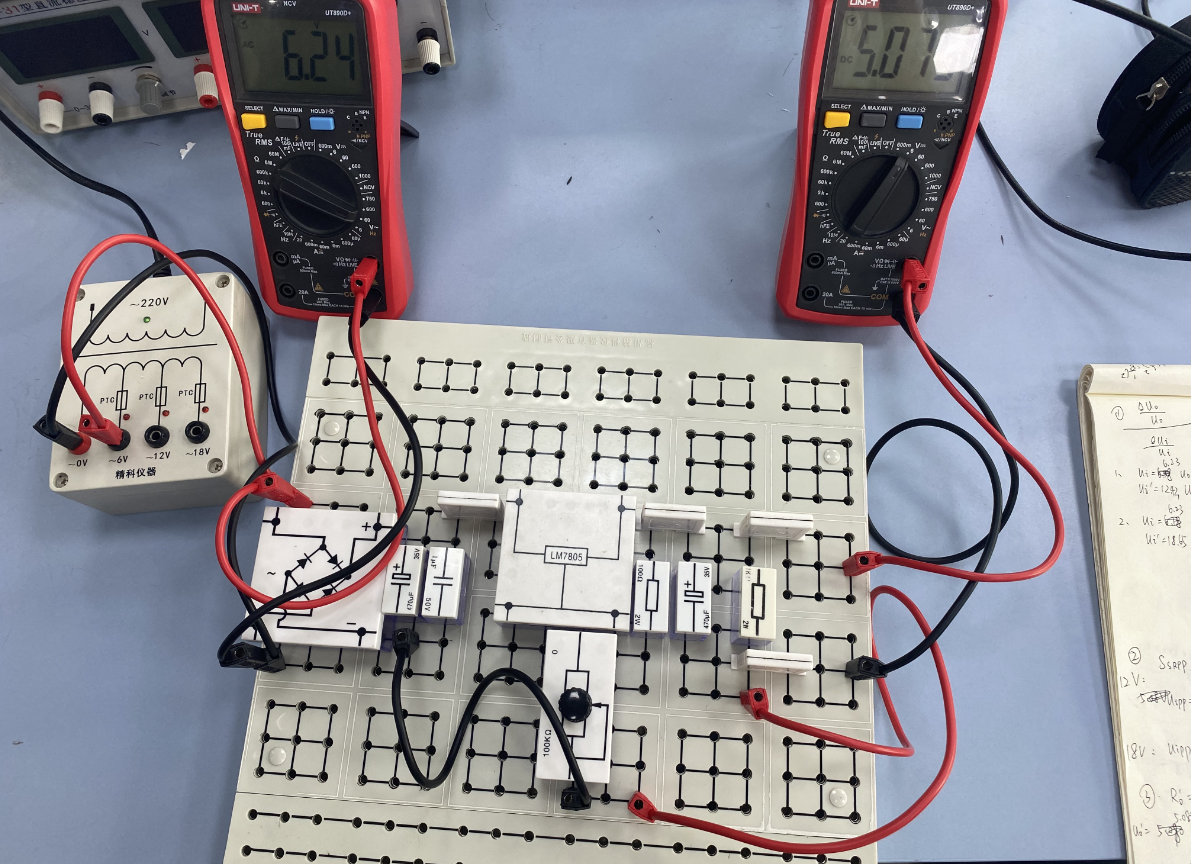
\includegraphics[clip,scale=0.6,trim={0 0 0 0}]{fig/fig1.png}
	        \caption{Related equipment display}
	        \label{figure.1}
    \end{figure}    
    
    \begin{itemize}
    \item \textbf{9-pin plugboard}: Provides a platform for connecting and arranging the components in the circuit.
    \item \textbf{AC power supply}: Supplies the alternating current (AC) voltage required for the experiment.
    \item \textbf{Digital multimeter}: Measures various electrical quantities such as voltage, current, and resistance in the circuit.
    \item \textbf{Capacitors}: Used for smoothing and filtering the output voltage of the voltage regulator.
    \item \textbf{Resistors} : Used for current limiting or voltage dividing purposes in the circuit.
    \item \textbf{Potentiometer}: Adjusts the output voltage of the voltage regulator circuit.
    \item\textbf{Diode}: Protects the circuit from reverse voltage or acts as a rectifier.
    \item \textbf{Three-terminal voltage regulator $(7805)$}: Maintains a constant output voltage regardless of changes in input voltage or load conditions.
    \item \textbf{Dual-trace oscilloscope}: Observes and measures the voltage waveforms in the circuit.
    \item\textbf{Connecting wires}: Used to establish electrical connections between the components and the circuit.
    \end{itemize}
    
        
	\section{Experimental principles}   
    \subsection{Circuit Composition}
    When the grid voltage changes or when the output load changes, the circuit that keeps the output voltage constant is called a voltage regulator. A DC regulated power supply is one of the most basic and commonly used instruments in electronic equipment. It is used as a source of energy to ensure the normal operation of electronic equipment.
    	\begin{figure}[H]
    	    	\centering
    	    	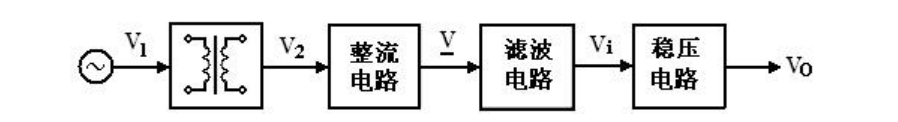
\includegraphics[clip,scale=1,trim={0 0 0 0}]{fig/fig2.png}
    	        \caption{Block diagram of DC voltage regulator circuit}
    	        \label{figure.2}
        \end{figure}    
    
    A DC regulated power supply generally consists of a rectifier circuit, a filter circuit and a voltage regulator circuit, as shown in Fig. fig-2. This experiment focuses on a DC regulated circuit consisting of a linear integrated voltage regulator 7805.
    	\begin{figure}[H]
    	    	\centering
    	    	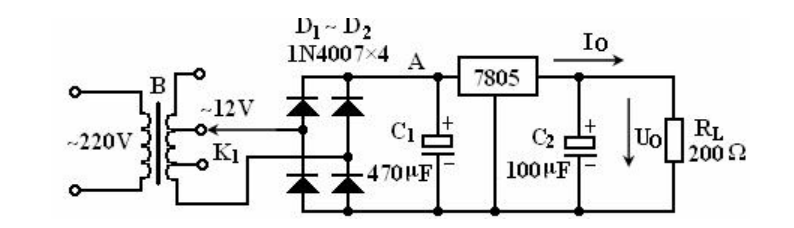
\includegraphics[clip,scale=1,trim={0 0 0 0}]{fig/fig3.png}
    	        \caption{Regulated circuit with fixed output of $5V$}
    	        \label{figure.3}
        \end{figure}   
    Figure fig-3 shows a regulated circuit with a fixed output of $5V$ consisting of a bridge rectifier, capacitor filter and 7805 linear regulator, while figure fig-4 shows an adjustable output regulator consisting of a bridge rectifier, capacitor filter and 7805 linear regulator. The function of each capacitor in the circuit is $C1$ is the filter capacitor, the capacitance and load current $I_0$ between the empirical formula is usually $\mathrm{C}_{1}=(1500 \sim 2000) \cdot \mathrm{I}_{0}(\mu \mathrm{F})$; $C2$ is the regulator self-oscillation suppression; $C3$ is the high frequency noise bypass capacitor
         
    	\begin{figure}[H]
    	    	\centering
    	    	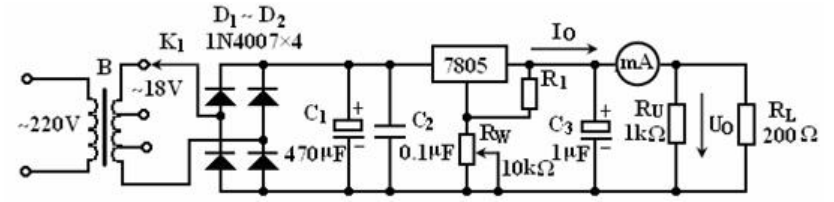
\includegraphics[clip,scale=1,trim={0 0 0 0}]{fig/fig4.png}
    	        \caption{Adjustable output voltage regulator}
    	        \label{figure.4}
        \end{figure}   
   
   \subsection{Rectifier circuits}
   \subsubsection{Half-wave rectification}
   The half-wave rectifier circuit is a simple electronic circuit for converting an AC signal into a unidirectional DC signal with the same frequency. It is based on the non-linear conducting characteristics of the diode, which allows current to pass in only one direction.

    	\begin{figure}[H]
    	    	\centering
    	    	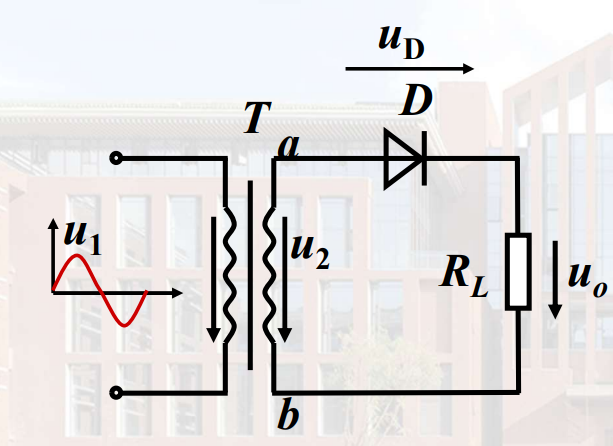
\includegraphics[clip,scale=0.8,trim={0 0 0 0}]{fig/fig5.png}
    	        \caption{Half wave rectifier circuit diagram}
    	        \label{figure.5}
        \end{figure}  
   
   The basic principle of a half-wave rectifier circuit is as follows:
   \begin{itemize}
   \item \textbf{Input signal}: The input of the half-wave rectifier circuit is an AC signal, typically sourced from an AC power supply or the secondary winding of a transformer. The input signal consists of alternating positive and negative half-cycles, with a frequency equal to the power supply frequency (usually 50Hz or 60Hz).
   
   \item \textbf{Diode}: The half-wave rectifier circuit includes at least one diode. Diodes have non-linear characteristics, where they conduct current when a forward voltage is applied and block current when a reverse voltage is applied.
   
   \item \textbf{Rectification process}: When the input signal voltage is positive, the diode is in the conducting state, allowing current to flow. In this case, the output circuit obtains a positive half-cycle waveform that is identical to the input signal. When the input signal voltage is negative, the diode is in the blocking state, preventing current flow, and the output circuit has no current flowing through it.
   
   \item \textbf{Output signal}: The output of the half-wave rectifier circuit is the rectified unidirectional DC signal. The amplitude of the output signal is the same as the positive half-cycle amplitude of the input signal, but it only contains the positive half-cycle portion.
   \end{itemize}
   
    	\begin{figure}[H]
    	    	\centering
    	    	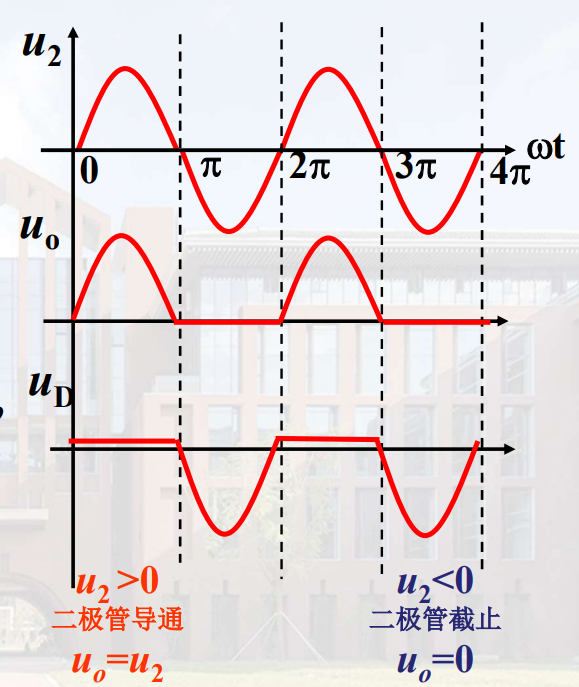
\includegraphics[clip,scale=0.65,trim={0 0 0 0}]{fig/fig6.png}
    	        \caption{Schematic diagram of the effect of a half-wave rectifier circuit}
    	        \label{figure.6}
        \end{figure}
        
    \begin{eqnarray}
    \begin{matrix}
    \textbf{DC voltage} \quad U_{0}&=&\frac{1}{2 \pi} \int_{0}^{2 \pi} u_{0} d(\omega t)=\frac{1}{2 \pi} \int_{0}^{\pi} \sqrt{2} U_{2} \sin \omega t d(\omega t)=\frac{\sqrt{2} U_{2}}{\pi}=0.45 U_{2}\\
    \textbf{DC current} \quad I_{0}&=&U_{0} / R_{L}=0.45 U_{2} / R_{L}\\
    \textbf{RMS current} \quad I_{2}&=&\sqrt{\frac{1}{2 \pi} \int_{0}^{\pi}\left(I_{2 m} \sin \omega t\right)^{2} d(\omega t)}=\frac{I_{2 m}}{2}=\frac{\pi I_{0}}{2}=1.57 I_{0}\\
    \textbf{Diode current} \quad I_{D}&=&I_{2} \quad I_{D 0}=I_{0}\\
    \textbf{Reverse voltage} \quad U_{D R M}&=&\sqrt{2} U_{2}
    \end{matrix}
    \end{eqnarray}
   
   \subsubsection{Single-phase full-wave rectification}
   Single-phase full-wave rectification is an electronic circuit used to convert an AC signal into a unidirectional DC signal. Compared to half-wave rectification, a single-phase full-wave rectification circuit makes more efficient use of the energy of the input signal, as it rectifies both the positive and negative half-periods of the input signal.

    	\begin{figure}[H]
    	    	\centering
    	    	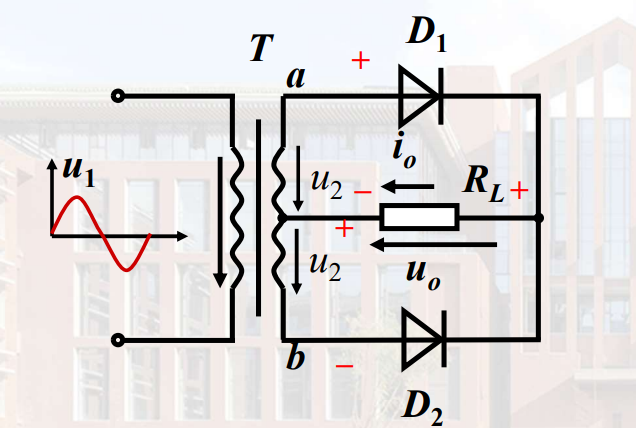
\includegraphics[clip,scale=0.8,trim={0 0 0 0}]{fig/fig7.png}
    	        \caption{Single-phase full-wave rectification diagram}
    	        \label{figure.7}
        \end{figure}  
   
   The basic principle of a half-wave rectifier circuit is as follows:
   \begin{itemize}
   \item \textbf{Input Signal}: The input of a single-phase full-wave rectifier circuit is an AC signal, usually sourced from an AC power supply or the secondary winding of a transformer. The input signal consists of alternating positive and negative half-cycles, with a frequency equal to the power supply frequency (typically 50Hz or 60Hz).
   
   \item \textbf{Rectifier Bridge}: The single-phase full-wave rectifier circuit utilizes a rectifier bridge, also known as a Graetz bridge, consisting of four diodes. Two diodes are connected to the positive half-cycle of the input signal, while the other two diodes are connected to the negative half-cycle. The rectifier bridge enables rectification of both positive and negative half-cycles of the input signal.
   
   \item \textbf{Rectification Process}: When the voltage of the input signal is positive, two diodes in the rectifier bridge are in a conducting state, allowing current to flow. In this case, the output circuit obtains a positive half-cycle waveform identical to the input signal. When the voltage of the input signal is negative, the other two diodes in the rectifier bridge are in a conducting state, and the output circuit still obtains a positive half-cycle waveform identical to the input signal.
   
   \item \textbf{Output Signal}: The output of the single-phase full-wave rectifier circuit is a rectified unidirectional DC signal. The amplitude of the output signal is the same as the amplitude of the positive half-cycle of the input signal, but it includes both positive and negative half-cycles of the input signal.
   
   \end{itemize}
   
    	\begin{figure}[H]
    	    	\centering
    	    	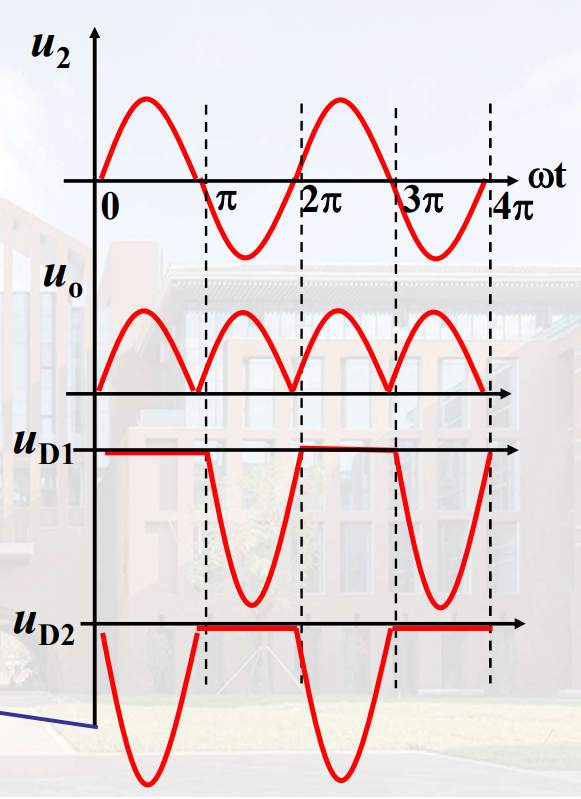
\includegraphics[clip,scale=0.65,trim={0 0 0 0}]{fig/fig8.png}
    	        \caption{Single-phase full wave rectifier waveform diagram}
    	        \label{figure.8}
        \end{figure}  
   
   Phase full wave rectification main parameters:
  \begin{eqnarray}
      \begin{matrix}
       U_{0}&=&\frac{1}{\pi} \int_{0}^{2 \pi} u_{0} d(\omega t)=\frac{1}{\pi} \int_{0}^{\pi} \sqrt{2} U_{2} \sin \omega t d(\omega t)=\frac{ 2\sqrt{2} U_{2}}{\pi}=0.9 U_{2}\\
       I_{0}&=&U_{0} / R_{L}=0.9 U_{2} / R_{L}\\
       I_{D0} &=& 0.5I_0\\
       I_{D}&=&I_{2} =1.57I_{D0}\\
       U_{D R M}&=&2\sqrt{2} U_{2}
      \end{matrix}
  \end{eqnarray}
   
  \subsubsection{Bridge rectifiers}
  Bridge rectification is an electronic circuit used to convert an AC signal into a unidirectional DC signal. It is achieved by using a bridge rectifier (also known as a full-wave bridge rectifier) to rectify both the positive and negative half-periods of the input signal.
  
  The bridge rectifier uses four diodes to form a bridge rectifier, which is similar in circuit construction to the rectifier bridge of a single-phase full-wave rectifier circuit. However, unlike the single-phase full-wave rectifier, the output circuit of the bridge rectifier is centred to ground (mid-point ground).

    	\begin{figure}[H]
    	    	\centering
    	    	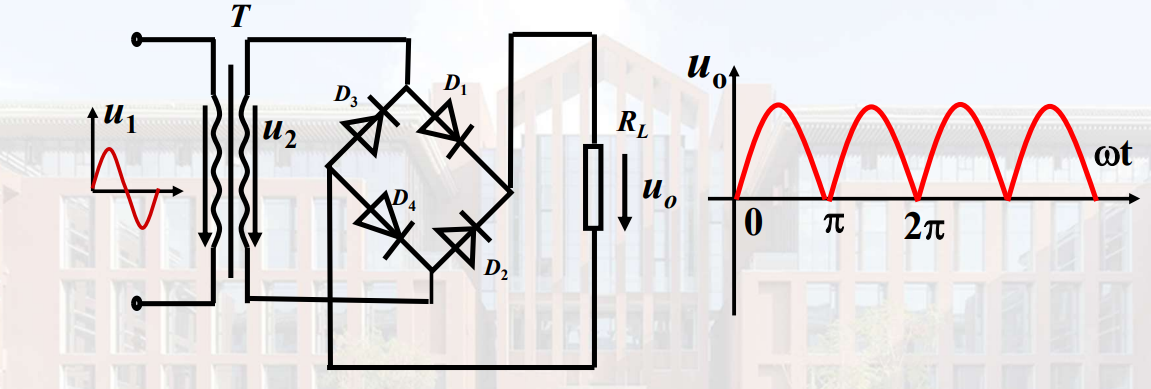
\includegraphics[clip,scale=0.65,trim={0 0 0 0}]{fig/fig9.png}
    	        \caption{Bridge rectifiers}
    	        \label{figure.9}
        \end{figure}
  
  \begin{itemize}
  \item Input Signal: The input of a bridge rectifier is an $AC$ signal, usually sourced from an $AC$ power supply or the secondary winding of a transformer. The input signal consists of alternating positive and negative half-cycles, with a frequency typically equal to the power supply frequency (e.g., $50Hz or 60Hz$).
  
  \item Bridge Rectifier: The bridge rectifier consists of a bridge rectifier bridge composed of four diodes. Two diodes are connected to the positive half-cycle of the input signal, while the other two diodes are connected to the negative half-cycle. This configuration allows the bridge rectifier to rectify both the positive and negative half-cycles of the input signal simultaneously.
  
  \item Rectification Process: When the voltage of the input signal is positive, two diodes in the bridge rectifier are in a conducting state, allowing current to flow. In this case, the output circuit obtains a positive half-cycle waveform identical to the input signal. When the voltage of the input signal is negative, the other two diodes in the bridge rectifier are in a conducting state, also allowing current to flow. Therefore, regardless of whether the input signal voltage is positive or negative, the output circuit obtains a positive unidirectional DC signal.
  
  \item Output Signal: The output of the bridge rectifier is a rectified unidirectional DC signal. The amplitude of the output signal is the same as the amplitude of the positive half-cycle of the input signal, but it includes both the positive and negative half-cycles of the input signal.
   
  \end{itemize}     
   
   \begin{eqnarray}
       \begin{matrix}
        U_{0}&=&\frac{1}{\pi} \int_{0}^{2 \pi} u_{0} d(\omega t)=\frac{1}{\pi} \int_{0}^{\pi} \sqrt{2} U_{2} \sin \omega t d(\omega t)=\frac{ 2\sqrt{2} U_{2}}{\pi}=0.9 U_{2}\\
        I_{0}&=&U_{0} / R_{L}=0.9 U_{2} / R_{L}\\
        I_{D0} &=& 0.5I_0\\
        I_{D}&=&I_{2} =1.57I_{D0}\\
        I_2 &=& \sqrt{2} 1.57I_{D0}\\
        U_{D R M}&=&2\sqrt{2} U_{2}
       \end{matrix}
   \end{eqnarray}    
  
  \subsubsection{Filter circuits}
  Structural features of filter circuits:
    	\begin{figure}[H]
    	    	\centering
    	    	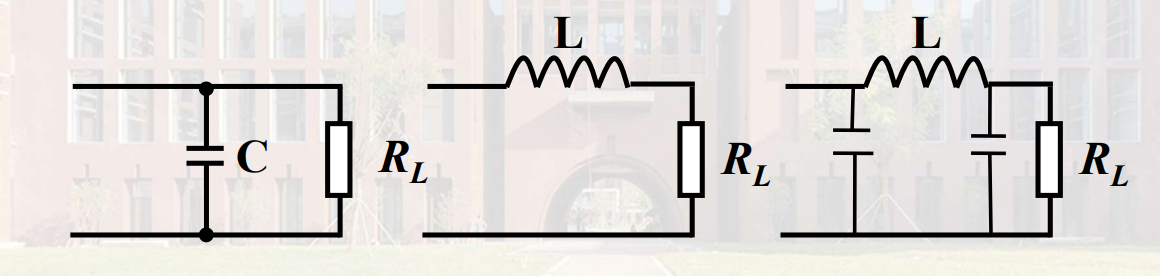
\includegraphics[clip,scale=0.65,trim={0 0 0 0}]{fig/fig10.png}
    	        \caption{Filter circuits}
    	        \label{figure.10}
        \end{figure}  
   Only if the rectifier circuit output voltage is greater than uc, there is a charging current The current The current in the diode is therefore a pulse wave. is a pulse wave.     
       
    \begin{figure}[H]
       \begin{minipage}[t]{0.6\linewidth}
          \centering
          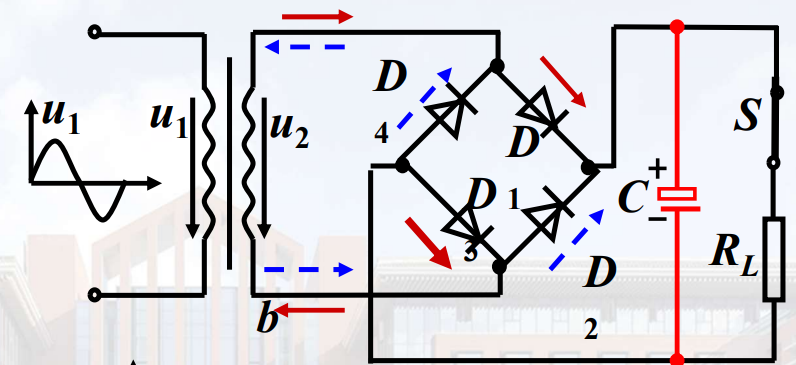
\includegraphics[clip,scale=0.6,trim={0 0 0 0}]{fig/fig11.png}
          \label{figure.11}
          \caption{Filter circuit schematic}
       \end{minipage}
       \begin{minipage}[t]{0.45\linewidth}
          \centering
          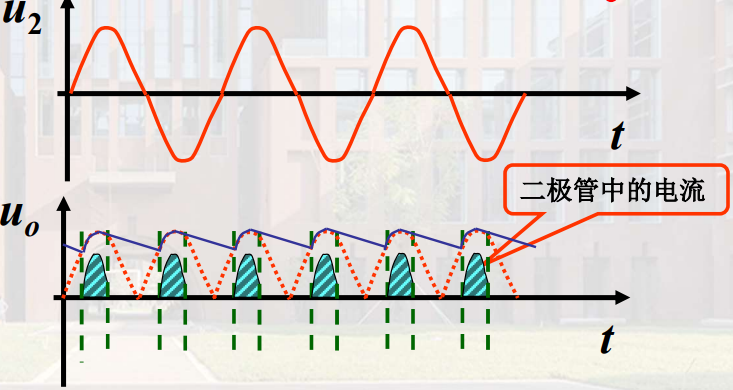
\includegraphics[clip,scale=0.55,trim={0 0 10 0}]{fig/fig12.png}
          \label{figure.12}
          \caption{Current in diodes}
       \end{minipage}   	  
    \end{figure}  
    
    Characteristics of capacitive filter circuits:
    \begin{itemize}
    \item The average value of the output voltage Uo is related to the time constant RLC.
    
    \item High transient current flow through the diode.
    
    \item Maximum reverse voltage to which the diode is subjected.
    \end{itemize}
    
    \subsection{Choice of circuit structure}  
    \textbf{Voltage regulator types}: linear series DC and switching regulators.
    \textbf{Voltage regulator components}: three-terminal regulators, transistor regulators, other integrated regulators.
    \textbf{Filter circuits}: capacitive filtering, inductive filtering, inductive-capacitive filtering.
    \textbf{ Rectifier circuits}: bridge rectifier, full wave rectifier, half wave rectifier.Frequency transformer step-down.
    
    The following circuit is obtained.

    	\begin{figure}[H]
    	    	\centering
    	    	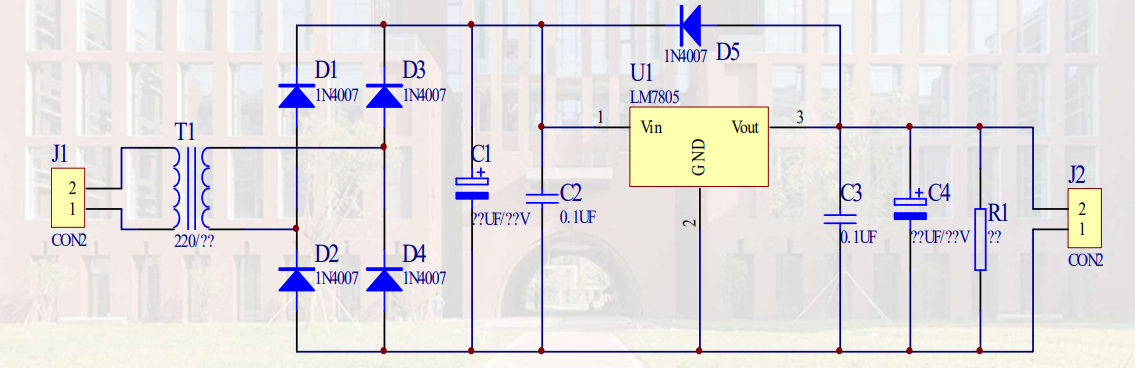
\includegraphics[clip,scale=0.8,trim={0 0 0 0}]{fig/fig13.png}
    	        \caption{Choice of circuit structure}
    	        \label{figure.13}
        \end{figure}  
        
    \subsection{Main indicator parameters of the voltage regulator circuit}
    Output voltage and its adjustable range: For adjustable regulated power supplies, the adjustable range of output voltage reflects the suitability of the application range of the power supply output. The range of application of the output reflects the suitability of the power supply.
    
    \textbf{The voltage stabilization factor $S_r$} : refers to the ratio of the relative change of the output voltage $U_0$ to the relative change of the input voltage $U_1$ when the load current and ambient temperature are constant in a $DC$ regulated power supply. The ratio of the relative change of the incoming voltage UI, expressed as:
    \begin{eqnarray}
    S_{r}=\frac{\Delta U_{\mathrm{o}} / U_{\mathrm{o}}}{\Delta U_{\mathrm{I}} / U_{\mathrm{I}}}
    \end{eqnarray}
    
    \textbf{Ripple Rejection Ratio $S_{SRPP}$} : The ripple rejection ratio is introduced to describe the performance of a voltage regulator circuit as the $AC$ component is not completely eliminated.It is defined as $20 \%$ of the logarithm of the ratio of the peak-to-peak input ripple voltage to the peak-to-peak output ripple voltage.
    \begin{eqnarray}
    S_{S \mathrm{RPP}}=20 \lg \frac{U_{\mathrm{ipp}}}{U_{\mathrm{OPP}}}
    \end{eqnarray}
    
    The higher the ripple rejection ratio, the better the regulator circuit is at eliminating the $AC$ component.
    
   \textbf{ Output resistance $R_0$} : defined as the ratio between the change in output voltage and the change in output current when the input voltage and ambient temperature do not change. The ratio between the change in output voltage and the change in output current when the input voltage and ambient temperature do not change. In experimental measurements, the output resistance is usually considered to be similar to the internal resistance of a power supply, measuring the open circuit output voltage o U' and the voltage across the load RL The output voltage $U_{0}^{'}$ and the voltage $U_0$ on the load $R_L$ can be measured using the formula:
   \begin{eqnarray}
   R_{\mathrm{o}}=\left(\frac{U_{o}^{\prime}}{U_{o}}-1\right) \cdot R_{\mathrm{L}}
   \end{eqnarray}
               
	\section{Contents and Steps}
	\begin{itemize}
	\item Step 1: Connect the circuit. After the circuit is connected, disconnect at point $A$ and measure and record the waveform of$U_1$(i.e., the waveform of $U$). Then, connect the circuit after point $A$ and observe the waveform of $U_0$. If there is any oscillation, it should be eliminated. Adjust$R_W$, and if the output voltage changes, the circuit is working properly.
    
    \item Step 2: Measure the output range of the voltage regulator. Adjust $R_W$ and use an oscilloscope to monitor the waveform of the output voltage $U_O$. Measure the maximum and minimum output voltages of the voltage regulator and their corresponding $U_1$ values. Measure the reference voltage of the voltage regulator (i.e., the voltage across the $100\Omega$  resistor).
    
    \item Step 3: Observe the ripple voltage. Adjust $R_W$ to make $U_0 = 5V$. Use an oscilloscope to observe the waveform of the input voltage $U_i$ of the voltage regulator and record the magnitude of the ripple voltage. Then, observe the ripple of the output voltage $U_O$ and compare the two.
    
    \item Step 4: Measure the output resistance $R_0$ of the voltage regulator. Disconnect $R_L$ ($R_L = \infty$) and measure the voltage across $R_L$, denoted as $U_O^{\prime}$. Then, connect $R_L$ and measure the corresponding output voltage $U_O$. Calculate $R_0$ using the following formula:
    
    \end{itemize}
    
   \begin{eqnarray}
   R_{\mathrm{o}}=\left(\frac{U_{o}^{\prime}}{U_{o}}-1\right) \cdot R_{\mathrm{L}}
   \end{eqnarray}

    	\begin{figure}[H]
    	    	\centering
    	    	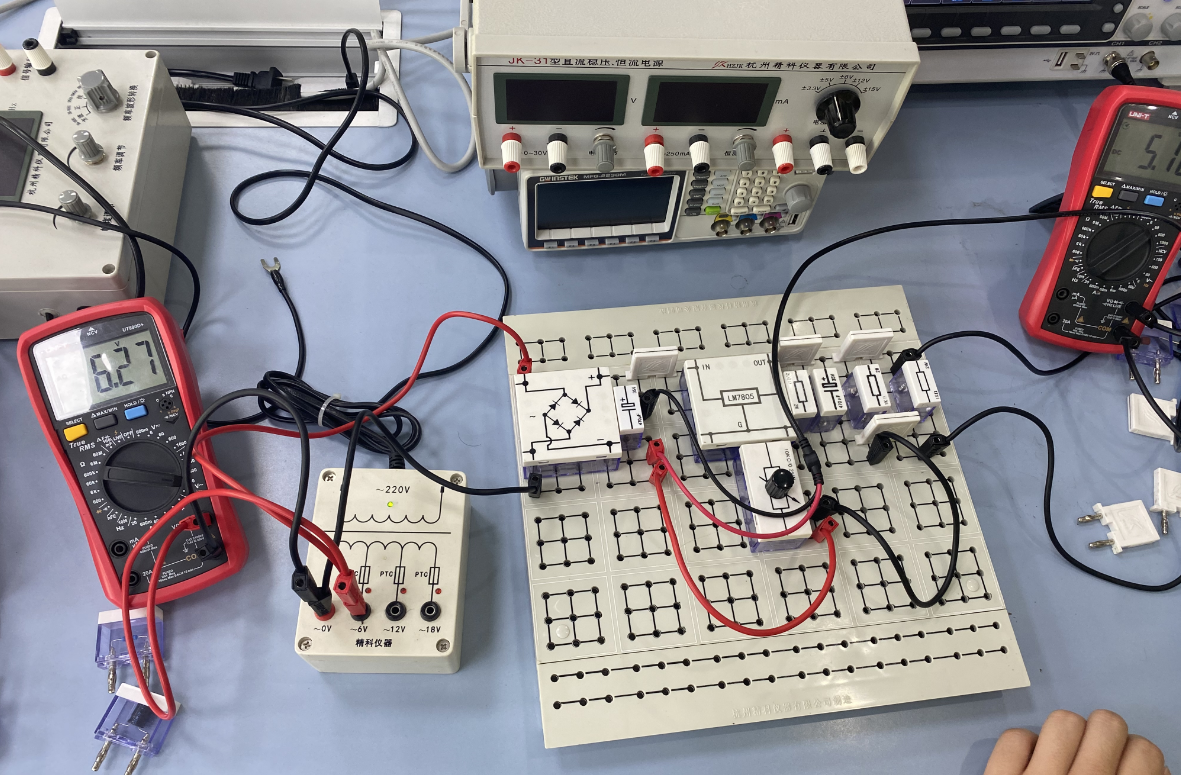
\includegraphics[clip,scale=0.5,trim={0 0 0 0}]{fig/fig14.png}
    	        \caption{Experimental manipulation diagram}
    	        \label{figure.14}
        \end{figure}      
	
	\section{Data processing}
   \subsection{Measurement and calculation of the voltage regulation factor}
   Based on the experimental content, we completed the measurement and recording of the voltage regulation coefficient and obtained the following data:
   \begin{table}[htbp]
     \centering
     \caption{Measurement Results Record Form}
       \begin{tabular}{lrrrrrrr}
       \toprule[2pt]
       index & \multicolumn{1}{l}{$u_0$} & \multicolumn{1}{l}{$u_{0}^{'}$} & \multicolumn{1}{l}{$\Delta u$}  & \multicolumn{1}{l}{$u_i$} & \multicolumn{1}{l}{$u_{i}^{'}$} & \multicolumn{1}{l}{$\Delta u_i$}  & \multicolumn{1}{l}{$S_r$} \\
       \midrule
       $6V \& 12V$ & 5.06  & 5.09  & 0.03  & 6.23  & 12.43 & 6.20   & 0.006 \\
       $6V \& 18V$ & 5.06  & 5.10   & 0.04  & 6.23  & 18.65 & 12.47 & 0.004 \\
       \bottomrule[2pt]
       \end{tabular}%
     \label{tab:addlabel}%
   \end{table}%
   
   Calculated from the formula:
       \begin{eqnarray}
       S_{r}=\frac{\Delta U_{\mathrm{o}} / U_{\mathrm{o}}}{\Delta U_{\mathrm{I}} / U_{\mathrm{I}}} =0.006 \quad or \quad 0.004
       \end{eqnarray}
       
   \subsection{Calculation of the ripple rejection factor}
    Based on the experimental content, we completed the measurement and recording of the voltage regulation coefficient and obtained the following data:
    
  \begin{table}[htbp]
    \centering
    \caption{Add caption}
      \begin{tabular}{lllr}
      \toprule[2pt]
      $U_i$  & $U_{ipp}$ & $U_{opp}$ & \multicolumn{1}{l}{$S_r$} \\
      \midrule
      12V   & 980mV & 40mV  & 27.8 \\
      18V   & 960mV & 60mV  & 24.2 \\
      \bottomrule[2pt]
      \end{tabular}%
    \label{tab:addlabel}%
  \end{table}%
    
   Calculated from the formula:
       \begin{eqnarray}
       S_{S \mathrm{RPP}}=20 \lg \frac{U_{\mathrm{ipp}}}{U_{\mathrm{OPP}}} = 27.8\quad or \quad 24.2
       \end{eqnarray}
       
   \subsection{Output resistance of the voltage regulator circuit}
   Based on the experimental content, we completed the measurement and recording of the voltage regulation coefficient and obtained the following data:
   
   \begin{table}[htbp]
     \centering
     \caption{Output resistance of the voltage regulator circuit}
       \begin{tabular}{rrrr}
        \toprule[2pt]
       \multicolumn{1}{l}{$R_L$} & \multicolumn{1}{l}{$U_{0}^{'}$} & \multicolumn{1}{l}{$U_0$} & \multicolumn{1}{l}{$R_0$} \\
       \midrule
       1000  & 5.08  & 5.075 & 0.99 \\
        \bottomrule[2pt]
       \end{tabular}%
     \label{tab:addlabel3}%
   \end{table}%
   
   Calculated from the formula:
    \begin{eqnarray}
      R_{\mathrm{o}}=\left(\frac{U_{o}^{\prime}}{U_{o}}-1\right) \cdot R_{\mathrm{L}} = 0.99
      \end{eqnarray}


\section{Conclusion and analysis}
\subsection{Conclusion}
Based on the above experiments, we finally obtained the experimental results: the regulator coefficients were $0.006$ and $0.004$, the ripple rejection coefficients were $27.8$ and $24.2$, and the output resistance of the regulator circuit was $0.99$

\subsection{Error analysis}
\begin{itemize}
\item \textbf{Measurement Errors}: The experiment involves various measurements, such as voltage measurements using a multimeter and waveform observations using an oscilloscope. Measurement errors can arise due to inaccuracies in the instruments, calibration issues, or human error while taking readings. It is important to consider the precision and accuracy of the measurement instruments and account for any uncertainties in the recorded values.

\item \textbf{Component Tolerances}: The performance of the voltage regulator circuit is influenced by the characteristics of its components, such as resistors, capacitors, and diodes. These components have tolerance values that specify the maximum allowable deviation from their nominal values. The actual values of the components used in the experiment may deviate from their ideal values, introducing errors in the circuit performance and output voltage regulation.

\item \textbf{Load Variations}: The voltage regulator circuit is designed to provide a stable output voltage under different load conditions. However, variations in the load resistance or current can affect the performance of the circuit and introduce deviations in the output voltage. It is important to note the range of load variations encountered during the experiment and analyze their impact on the voltage regulation and stability.

\item \textbf{Ripple and Noise}: Voltage regulators aim to minimize ripple and noise in the output voltage. However, due to the inherent characteristics of the circuit and external factors, some amount of ripple and noise may still be present in the output. These fluctuations can result from power supply imperfections, component tolerances, or electromagnetic interference. Analyzing the magnitude of ripple and noise and their impact on the output voltage stability is crucial in assessing the performance of the voltage regulator circuit.

\item \textbf{Design Limitations}: The design of a voltage regulator circuit involves selecting appropriate components, determining their values, and configuring the circuit to meet specific requirements. However, certain design limitations, such as power dissipation, voltage drop across components, or maximum current handling capacity, may impose constraints on the circuit's performance. Evaluating these design limitations and their effects on the circuit's behavior is important for a comprehensive analysis of the voltage regulator's characteristics.
\end{itemize}

\begin{appendix}
\section{Experimental procedure diagram}
    	\begin{figure}[H]
    	    	\centering
    	    	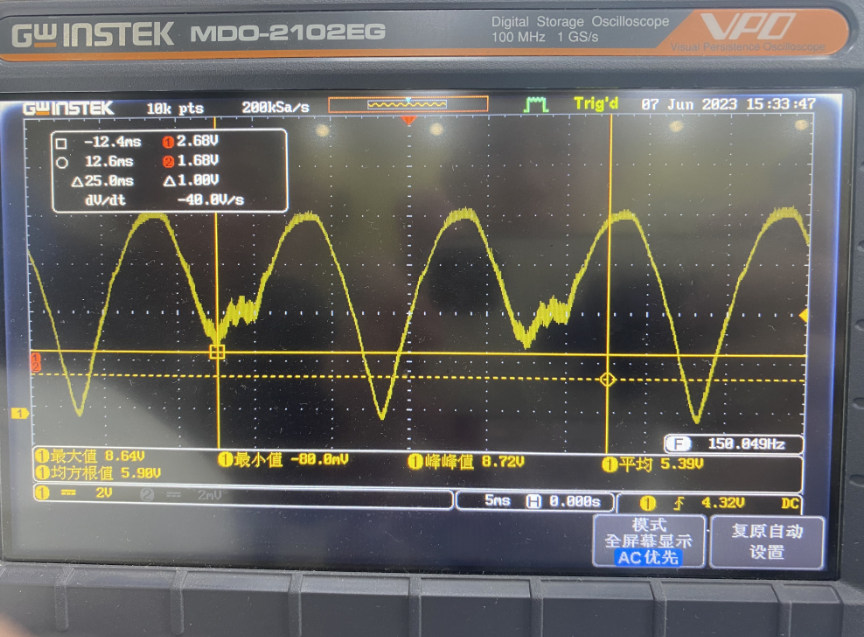
\includegraphics[clip,scale=0.8,trim={0 0 0 0}]{fig/fig15.png}
    	        \caption{Rectification schematic}
    	        \label{figure.15}
        \end{figure}  

    	\begin{figure}[H]
    	    	\centering
    	    	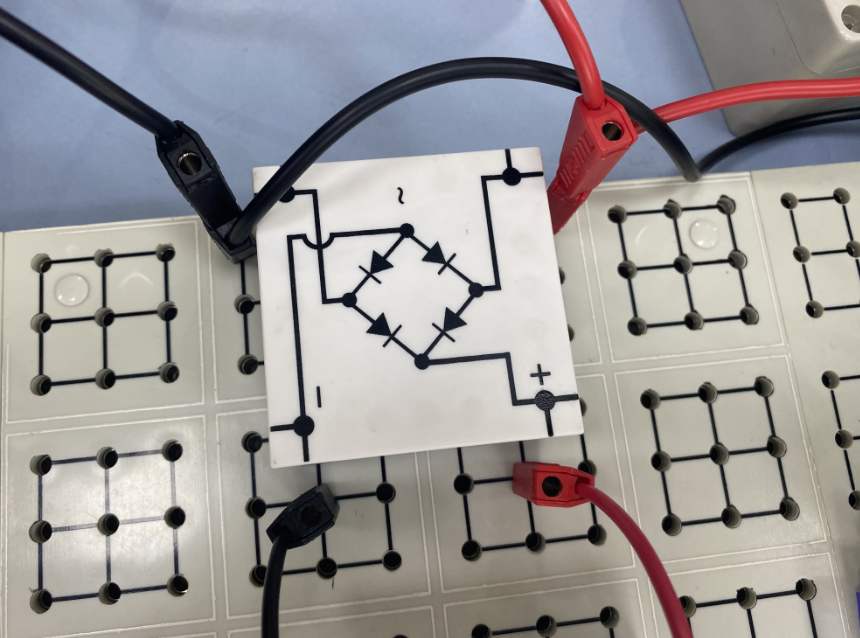
\includegraphics[clip,scale=0.8,trim={0 0 0 0}]{fig/fig16.png}
    	        \caption{Schematic diagram of the bridge link}
    	        \label{figure.16}
        \end{figure}          

    	\begin{figure}[H]
    	    	\centering
    	    	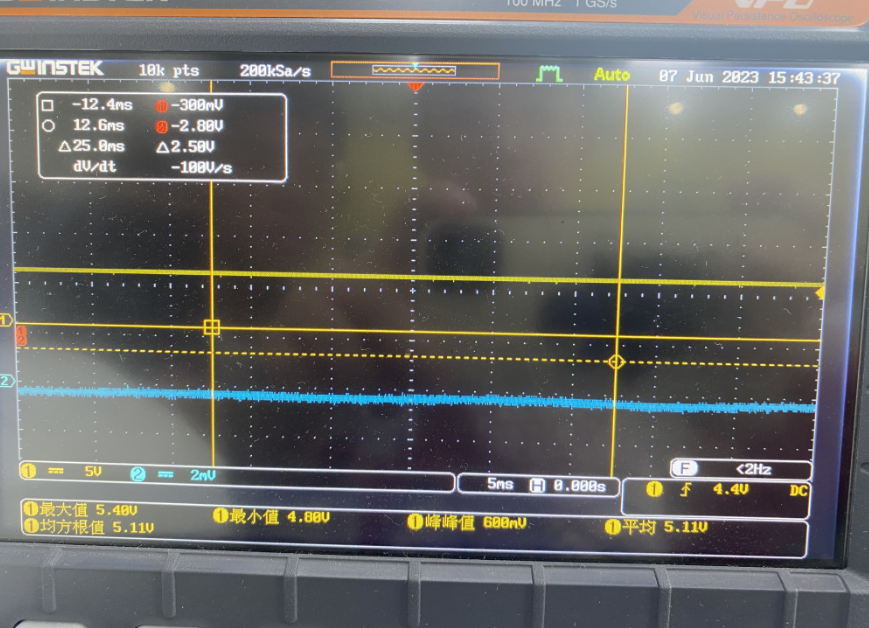
\includegraphics[clip,scale=0.8,trim={0 0 0 0}]{fig/fig17.png}
    	        \caption{Waveform diagram after rectification, filtering and stabilisation}
    	        \label{figure.17}
        \end{figure}  
        
    	\begin{figure}[H]
    	    	\centering
    	    	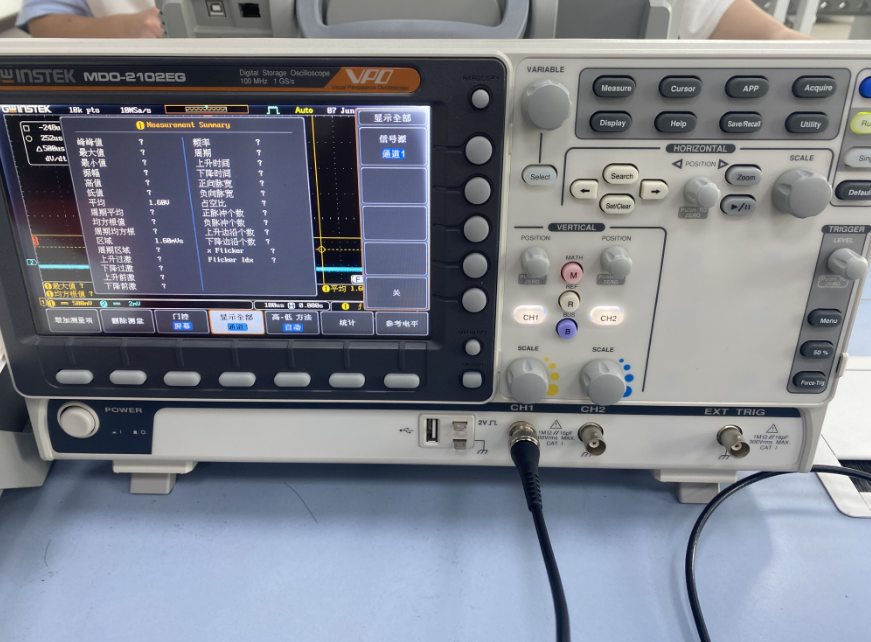
\includegraphics[clip,scale=0.8,trim={0 0 0 0}]{fig/fig18.png}
    	        \caption{Measurement data recording chart}
    	        \label{figure.18}
        \end{figure} 
        
 \section{Experimental data recording graph} 
     	\begin{figure}[H]
     	    	\centering
     	    	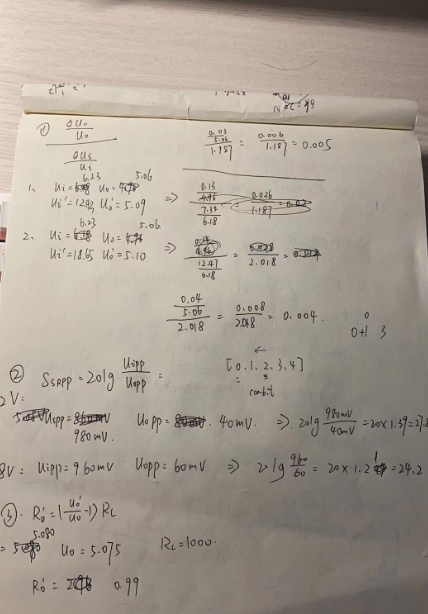
\includegraphics[clip,scale=1.6,trim={0 0 0 0}]{fig/fig19.png}
     	        \caption{Experimental data recording graph}
     	        \label{figure.19}
         \end{figure} 
 \end{appendix}        
\end{document}  